\documentclass[12pt,a4paper,twoside,openright]{book}

%%%%%%%%%%%%%%%%%%%%%%%%%%%%%%%%%%%%%%%%%%%%%%%%%%%%%%%%%%%%%%%%%%%%
%  Template per Tesi di Laurea                                     %
%                                                                  %
%%%%%%%%%%%%%%%%%%%%%%%%%%%%%%%%%%%%%%%%%%%%%%%%%%%%%%%%%%%%%%%%%%%%

               %%%%%%%%%%%%%%%%%%%%%%%%%%%%%%%%%%%%%%
               %    Scelta dei package da usare     %
               %%%%%%%%%%%%%%%%%%%%%%%%%%%%%%%%%%%%%%


\usepackage[dvips]{graphicx}
\usepackage{graphics}
\usepackage[normalem]{ulem}
\usepackage[utf8]{inputenc}
\usepackage[italian,british]{babel}
\usepackage{float}
\usepackage{graphicx,algorithm,algorithmic}
\usepackage{amsmath,amsfonts,amssymb,amsthm}
\usepackage{epsfig}
\usepackage{deistesi}
\usepackage{fancyhdr}
\usepackage{xspace}
\usepackage[colorlinks=false]{hyperref}
\usepackage[avantgarde]{quotchap}
\renewcommand\chapterheadstartvskip{\vspace*{-5\baselineskip}}
\renewcommand\sectfont{\sffamily\bfseries}
\usepackage{mathptmx}       % selects Times Roman as basic font
\usepackage{helvet}         % selects Helvetica as sans-serif font
\usepackage{courier}        % selects Courier as typewriter font
\usepackage{type1cm}        % activate if the above 3 fonts are
\usepackage{makeidx}         % allows index generation
\usepackage{multicol}        % used for the two-column index
\usepackage[bottom]{footmisc}% places footnotes at page bottom
\usepackage{times}
\usepackage{subfigure}
\usepackage{stmaryrd,mathtools}
\usepackage{eurosym}
\usepackage{cleveref}


\newcommand{\bnfs}[0]{\;|\;}
\newcommand{\opar}[0]{\;|\;}
\newcommand{\sq}[0]{\oplus}
\newcommand{\tuple}[2]{#1\langle #2\rangle}
\newcommand{\tupled}[2]{#1[#2]^{\Rightarrow}}
\newcommand{\actrate}[2]{#1^{#2}}
\newcommand{\leave}{{}}
\newcommand{\near}[3]{#1\!\stackrel{#3}{\rightsquigarrow}\!#2 }
\newcommand{\scope}[2]{\llbracket #1 \rrbracket_{#2}}
\newcommand{\law}[1]{[#1]}
\newcommand{\firing}[3]{#1^\rightsquigarrow(#2,#3)}
\newcommand{\shfiring}[1]{#1^\rightsquigarrow}

\newcommand{\defn}[2]{\mathit{def} #1 := #2}
\newcommand{\defnarr}[2]{\mathit{def} #1 & := & #2}
\newcommand{\call}[1]{call\, #1}


               %%%%%%%%%%%%%%%%%%%%%%%%%%%%%%%%%%%%%%
               %  Scelta del tipo di font da usare  %
               %%%%%%%%%%%%%%%%%%%%%%%%%%%%%%%%%%%%%%

%\usepackage{times,mathptm}
%\usepackage{palatino,mathpple}
%\usepackage{bookman}
%\usepackage{newcent}

               %%%%%%%%%%%%%%%%%%%%%%%%%%%%%%%%%%%%%%%%
               % Scelta delle dimensioni della pagina %
               %%%%%%%%%%%%%%%%%%%%%%%%%%%%%%%%%%%%%%%%

\setlength{\textwidth}{16.0cm}
\setlength{\textheight}{21cm}
\setlength{\footskip}{3cm}



               %%%%%%%%%%%%%%%%%%%%%%%%%%%%%%%%%%%%%%
               %  Informazioni generali sulla Tesi  %
               %    da usare nell'intestazione      %
               %%%%%%%%%%%%%%%%%%%%%%%%%%%%%%%%%%%%%%

\titolo{Engineering complex computational ecosystems}
\candidato{Danilo Pianini}
\annoaccademico{2015}
\facolta{Ingegneria}
\dipartimento{DEIS - Dipartimento di Elettronica, Informatica e Sistemistica}
\dottorato{PhD Course in Electronics, Computer Science and Telecommunications}
\settoreconcorsuale{09/H1}
\settoredisciplinare{ING-INF/05}
\ciclo{XXVII}
\tutor{Antonio Natali}
\relatore{Mirko Viroli}
% \correlatoreb{Andrea Roli}
% \correlatorec{Mirko Viroli}
\coordinatore{Alessandro Vanelli Coralli}
\dedica{
\emph{\mbox{~~~~~~~~~~~~~~~~~~~~~~~~~~~~~~~~~~~~~~~}Lorem ipsum dolor sit amet. \\
%
\mbox{~~~~~~~~~~~~~~~~~~~~~~~~~~~~~~~~~~~~~~~~~~~~}consectetur adipiscing elit.\\
%
\mbox{~~~~~~~~~~~~~~~~~~~~~~~~~~~~~~~~~~~~~~~~~~~~}Sed fringilla quis mauris id sagittis everything.}\\ \\ \\ \\
\noindent \emph{\textbf{Acknowledgements}}\\ \\
Curabitur commodo dictum risus laoreet tincidunt. Sed dapibus nec ex sit amet consequat. Quisque cursus est sit amet lectus tempor, nec egestas sapien rutrum. Sed dapibus consequat egestas. Quisque blandit, tellus et molestie interdum, augue est molestie lorem, tristique congue metus massa sed eros. Vivamus fermentum erat a faucibus porta. Praesent sit amet risus leo. Integer venenatis lectus sed euismod euismod. Ut pulvinar fermentum sagittis. Aliquam maximus nisl velit, ac varius tellus dignissim in. Fusce nibh dolor, blandit vel nisl non, vehicula tincidunt lorem. Suspendisse fringilla magna ac justo fermentum, nec accumsan odio sollicitudin. Maecenas consectetur, nulla sit amet ultricies pretium, metus sapien posuere turpis, in lobortis tellus turpis ac ipsum. Aliquam sollicitudin augue a aliquam volutpat. Mauris bibendum nunc id est ullamcorper, nec feugiat elit dapibus.\\
%
Duis tincidunt maximus justo, id convallis mauris mattis congue. Maecenas ullamcorper laoreet lacinia. Praesent luctus dictum metus, sed ultrices dui. Fusce fringilla eu est sit amet porta. Aliquam ornare eleifend congue. Aliquam orci urna, accumsan nec metus a, tincidunt pulvinar augue. Nunc eu vulputate lectus. Morbi placerat varius purus at scelerisque. Mauris malesuada ut massa non porta. Quisque ac efficitur odio. Aliquam scelerisque dapibus felis in ullamcorper. Pellentesque ullamcorper massa quis nibh suscipit elementum. Suspendisse tincidunt, sem non porta consectetur, arcu mauris mollis mi, ut commodo libero diam ut risus.
}
\data{March 2015}
\signature{\emph{Danilo Pianini}}

              %%%%%%%%%%%%%%%%%%%%%%%%%%%%%%%%%%%%%%
               % Fine Preambolo                     %
               % Inizio tesi                        %
               %%%%%%%%%%%%%%%%%%%%%%%%%%%%%%%%%%%%%%

\begin{document}

%%%%%%%%%%%%%%%%%%%%%%%%%
% inizio prefazione
%
% pagina del titolo, indice, sommario
%%%%%%%%%%%%%%%%%%%%%%%%%
\frontmatter
\maketitle
\pagestyle{plain}
\tableofcontents

\chapter*{\centering Abstract}
\addcontentsline{toc}{chapter}{Abstract}

This work presents advancements of the latest three years in the engineering techniques for self-organising pervasive ecosystems of devices and services.
%
The inherent complexity of such systems poses new challenges to those who try to dominate the complexity by applying the principles of engineering.

The recent growth in number and distribution of devices with decent computational and communicational abilities, that got suddenly accelerated with the massive diffusion of smartphones and tablets, is envisioning a world with a much higher density of devices in space.
%
This already high device density is probably going to consistently rise if the diffusion of wearable devices gets momentum.
%
Also, communication technologies seem to be focussing on short-range device-to-device (P2P) interactions, with technologies such as \btle{} and Near-Field Communication getting more and more diffused.

Locality and situatedness become key to provide the best possible experience to users, and the classic model of a centralised, enormously powerful server gathering data and processing it is likely to get less and less efficient with device density.
%
Accomplishing complex global tasks without a centralised controller responsible of aggregating data from devices, however, still is a challenging task.
%
In particular, it is hard to understand which device-local programs could properly interact and guarantee a certain global service level.
%
Such local-to-global issue makes the application of engineering principles challenging at least.

In this work, I lay the foundations of my contribution by first analysing the state of the art in coordination systems, namely in those software frameworks devoted to control and promote interactions among independent software entities.
%
I then motivate my work, by describing the main issues of pre-existing tools and practices and identifying the improvements that would benefit the design of such complex software ecosystems.
%
My contribution is described in \Cref{contribution}, and can be divided in three main branches: i) a novel simulation tool for pervasive ecosystems, ii) introduction of novel and improvements over existing self-organisation patterns, iii) the creation of a new language and interpreter based on ``field calculus'' and its integration with the previously mentioned simulator.
%
Finally, I draw conclusions and future works.

\mainmatter

% stile della pagina
\pagestyle{fancy}
\fancyhead[LE,RO]{\bfseries\thepage}

\part{Background and Motivation}
\label{background}
\chapter{Pervasive devices}
\label{pervasive-devices}

It is no mystery that, with the huge progresses of miniaturisation, computational-capable devices are populating the world.
%
The diffusion got momentum with affordable ``personal computers'' that made their way in a one-device-per-family world.
%
Laptops boosted the process, offering user a personal and mobile device.

The pervasive revolution, however took place when the phones became ``smart'', and with the subsequent improvements in the communication technologies.
%
In this chapter, I try to briefly walk the path of success of personal mobile devices, describing also the probable newcomer, namely the wearable devices.
%
I also focus on the current status of the communication protocols, their range and usage, and I try to foresee which world are we going to build if the current trend continues.

\section{Smart, portable devices}

\begin{figure}
	\centering
	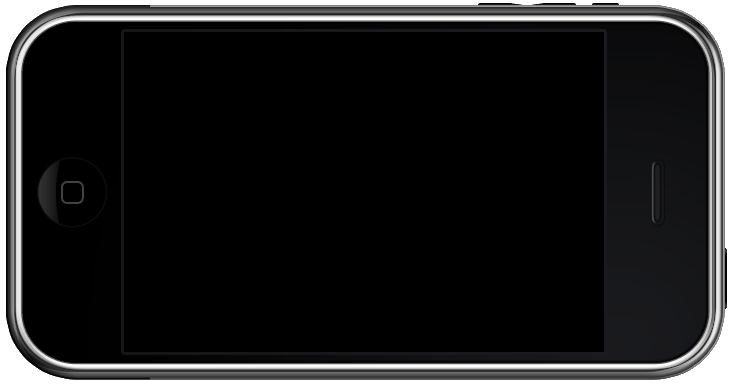
\includegraphics[width=0.99\textwidth]{img/iphone}
	\caption{Apple iPhone is one of the first devices without any physical keyboard, and the first smartphone to gain worldwide success. \emph{Source: Wikimedia.}}
	\label{img:iphone}
\end{figure}

When Apple in 2007 released the first iPhone (\Cref{img:iphone}), a mobile revolution started.
%
Even though other manufacturers proposed products similar to iPhone under the point of view of communication technologies and computational capabilities in the same time frame (e.g. Nokia N810), the Apple's smartphone was the first gaining widespread adoption.
%
It is not really relevant for this work to understand if the branding, the design, the multi-touch finger based interaction UI or the feature set was the key of its commercial success: what really matters is that, starting 2007, every person began to carry with her a personal device featuring both the abilities to communicate and compute.
%
The reason, besides the success of iPhone in the higher segment of the phone market, is mainly to attribute to the widespread diffusion of similar but cheaper and less powerful devices in the lower segments.
%
This kind of devices ultimately pushed the market share of the dominating today's mobile operating system, Google's Android.

This trend towards a higher diffusion got another leap forward three years later, in 2010, when a device with a feature set similar to iPhone, but with no phone abilities  and a bigger screen was released: the iPad.
%
As iPhone gave new vitality and perspectives to the phone arena, iPad revitalised a market that was languishing: the tablets.
%
Tablet devices as they were conceived before iPad launched were nothing more than small laptops with a screen that could be rotated or detached from the keyboard, and a touch-screen normally used with the help of a pen.
%
They changed from devices designed for a professional niche to widespread tools, up to the point that Gartner forecasts their shipments to overtake in 2015 those of desktop PC and laptops aggregated \footnote{\url{http://www.gartner.com/newsroom/id/2791017}}.

The new frontier of pervasive is probably the wearable technology. Smartphones were precursors, they substituted mobile phones introducing new features and they have potential to substitute our wallets (see, for instance, payments through NFC technology) and keys, becoming the only object we need to carry with us in our pockets.
%
Still there are other accessories which are hard to replace, above all watches and glasses.
%
Yes, smartphone can easily show the current time accurately (and, to be honest, also feature phones had this feature well before 2007), but they require the user to pick them from the pocket, turn them on, and sometimes, depending on privacy settings, also unlock them.
%
The whole operation, takes a much longer time and higher effort with respect to just rotating a wrist.
%
This might be the reason why, despite the explosive expansion of smartphones, the wristwatches market did not declined, as an analysis from MarketWatch points out \footnote{\url{http://www.marketwatch.com/story/the-watchs-time-isnt-up-2013-07-01}}.

\begin{figure}
	\centering
	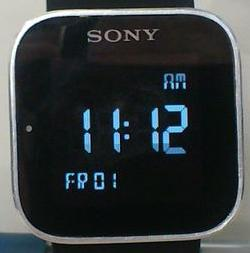
\includegraphics[height=5cm]{img/sony-sw}
	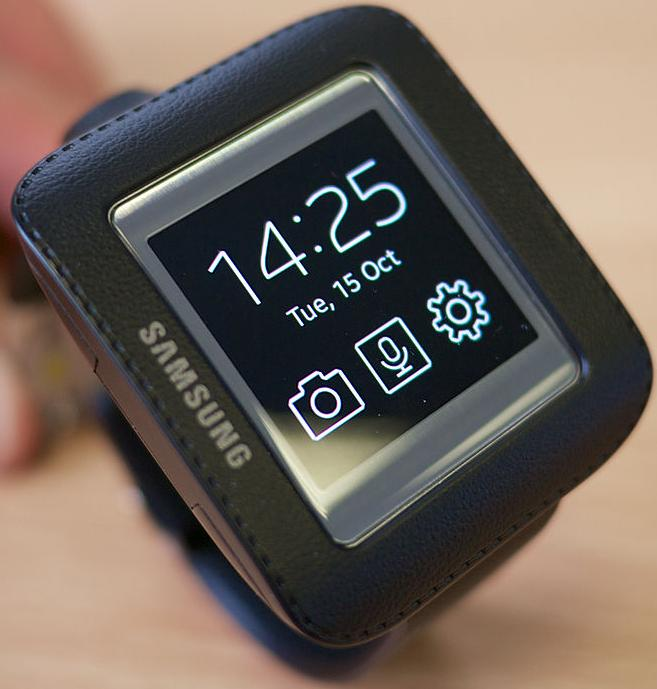
\includegraphics[height=5cm]{img/samsung-gg}
	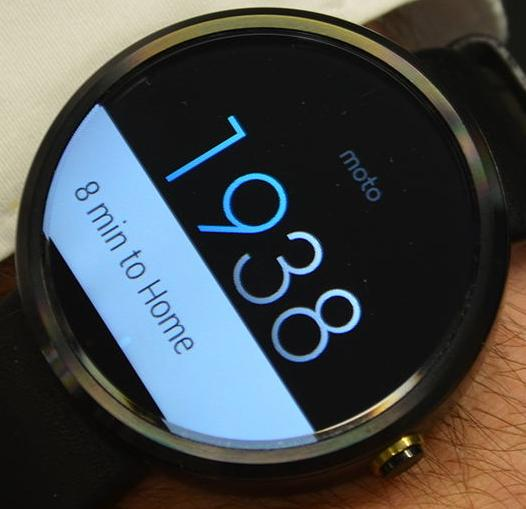
\includegraphics[height=5cm]{img/moto360}
	\caption{Smart watches. From left to right: Sony Smartwatch \emph{(Source: Alex S.H. Lin)}, Samsung Galaxy Gear \emph{(Source: Karlis Dambrans)}, Motorola Moto 360.}
	\label{img:watches}
\end{figure}

There is room for manufacturers to create new portable devices.
%
Sony, starting 2012, has produced a series of smartwatches, such as those in \Cref{img:watches} that pair with a smartphone and provide quick access to some of its functionalities.
%
The success of such solution is not huge, but despite that many other companies are interested in this market: Samsung, Motorola and Apple presented devices meant to replace the classic wristwatch, a clear sign that this market is in expansion.
%
At the time of writing, the main issues that slow the widespread adoption of such solutions are battery duration and dependence on a smartphone.

\begin{figure}
	\centering
	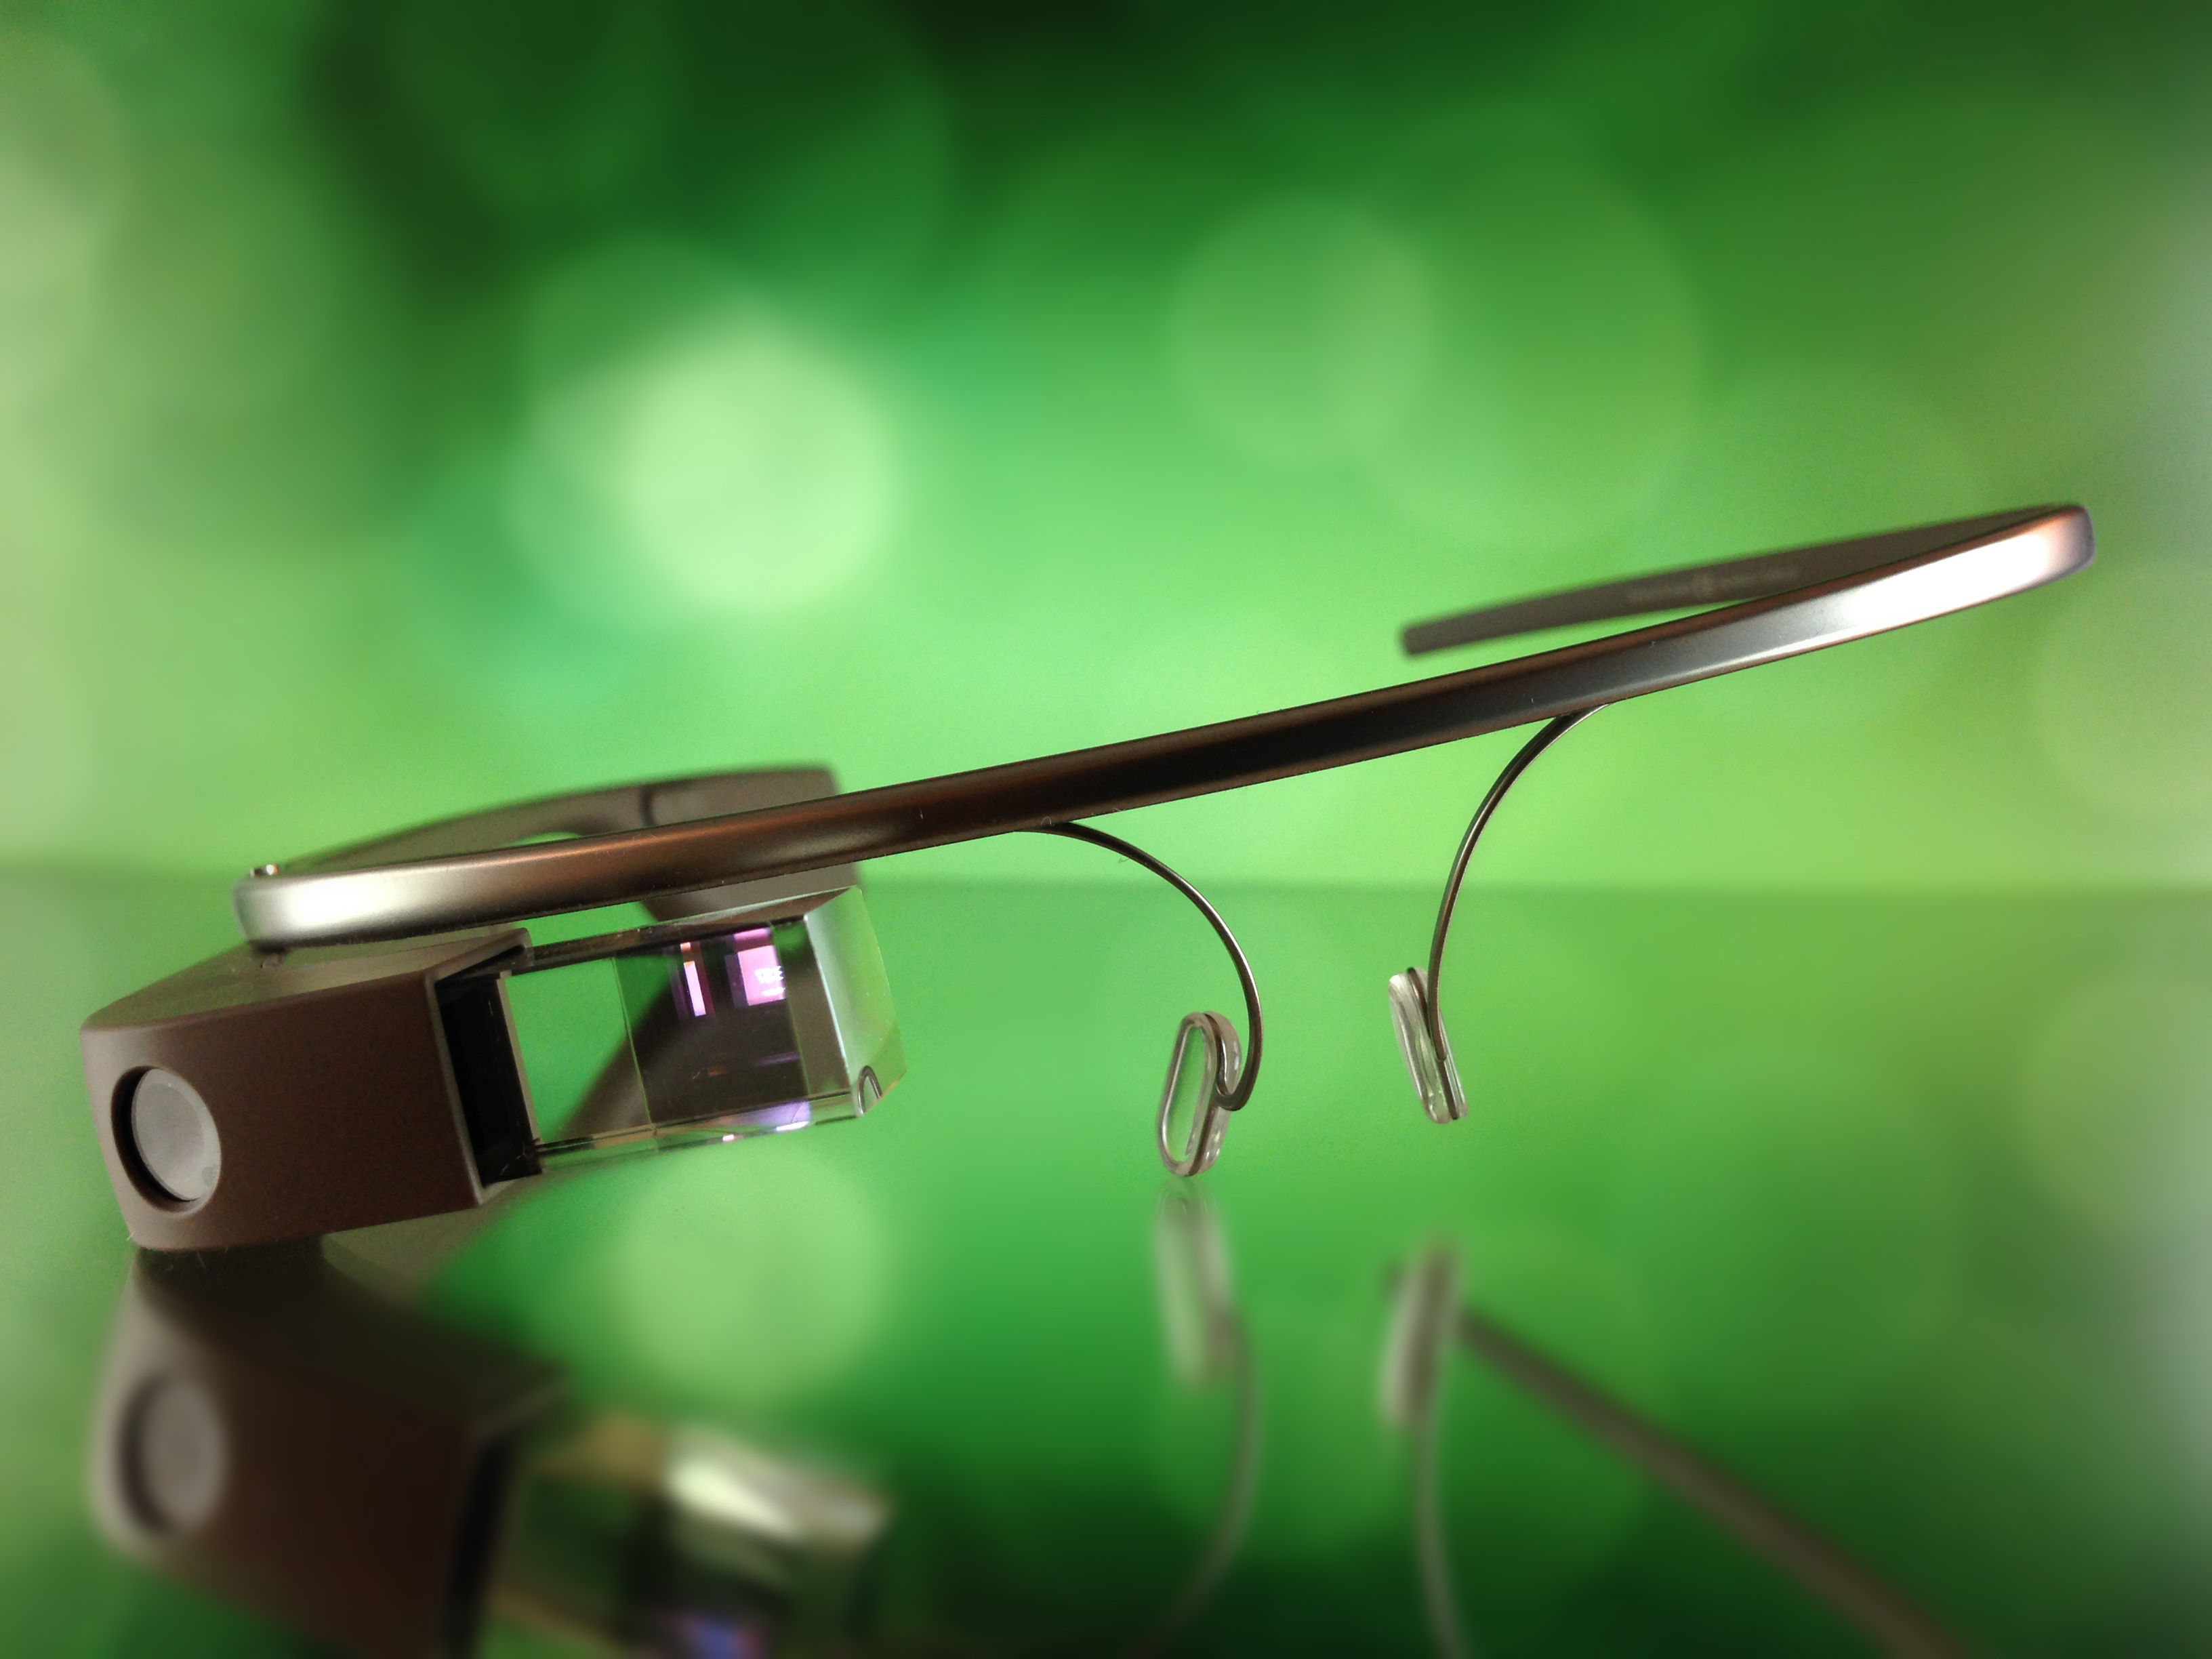
\includegraphics[width=0.99\textwidth]{img/gglass}
	\caption{Google Glass. In this image, it is possible to see both the camera (on the left hand side) and the semi-transparent head-mounted display. Are those devices going to be part of our everyday life? \emph{Source: Wikimedia.}}
	\label{img:gglass}
\end{figure}

Another notable attempt to make a common accessory smarter is Google Glass project, depicted in \Cref{img:gglass}.
%
Their goal is to enhance the experience of wearing glasses by attaching a device with a camera, an optical head-mounted display, and the abilities to locate itself and communicate with other devices.
%
Google Glass, at the time of writing, are way to expensive (with the kit sold at \$1500) for being able to penetrate the general public, but they are an interesting anticipation of possible future devices.

On the same line of such wearable devices, a discrete success is being achieved by the so called ``fit bands''.
%
They are bracelets equipped with low energy sensors, mainly accelerometers and gyroscopes, which are used to keep track of user's activity.
%
Depending on the model, they can be used to monitor some user's health parameters, such as the number of steps walked per day or heartbeats.
%
They normally work along with another device, a smartphone or a tablet.
%
Such devices, due to their precise market niche and reasonably low price (the Chinese manufacturer Xiaomi recently introduced a low-end wristband at around \$15) are having a notable success.

The wearable devices segment also includes less common devices such as ``smart shoes'' and materials that can be used to make clothing, such as e-textiles.
%
It is a market in expansion, greatly beneficing from recent increases in performance per watt efficiency.
%
If the trend continues, it is likely that we will more and more powerful wearable devices on sale at cheaper and cheaper prices, and a consequent widespread diffusion.
%
The same sort may occur to other parts of our life: kitchen gear, indoor lights and many other objects are getting more and more ``smart'' around us.
%
We may, literally, end up with a world where every single object embeds computational and communicational abilities.

A problem arise: how can software engineers deal with such a complexity?

\section{Communication technologies}

Besides miniaturisation, and as a consequence the increase of computational density in space, another factor played a fundamental role in the world of pervasive computing: the ability to communicate, and in particular the ability to rely on wireless communication, which is of paramount importance when considering mobility.

In later years, many communication means arose.
%
They largely differ in terms of range, protocols, and availability.
%
In this section, I try to resume the most diffused technologies available on today's devices, but the reader is warned: keep in mind that such technologies are evolving very quickly, and the scenario is incredibly fluid.

\subsection{International Mobile Telecommunications}
\label{International Mobile Telecommunications}

This first mean of communication is designed to allow mobile devices to access the Internet from anywhere in the world, relying on the existing mobile phone infrastructure.
%
Such technologies are meant to be used with the standard IP protocols, and they are normally used to get access to public services, in particular to the world wide web.
%
They are not designed for a local peer-to-peer (P2P) communication, and as a consequence they provide no mean to exploit locality.
%
The diffusion of such communication protocols is widespread, in particular among smartphones.
%
Due to the fact that they rely on the mobile phone network, they require a contract with a mobile telecommunications provider, and as such they are much less diffused in tablets and other portable devices.

\begin{figure}
	\centering
	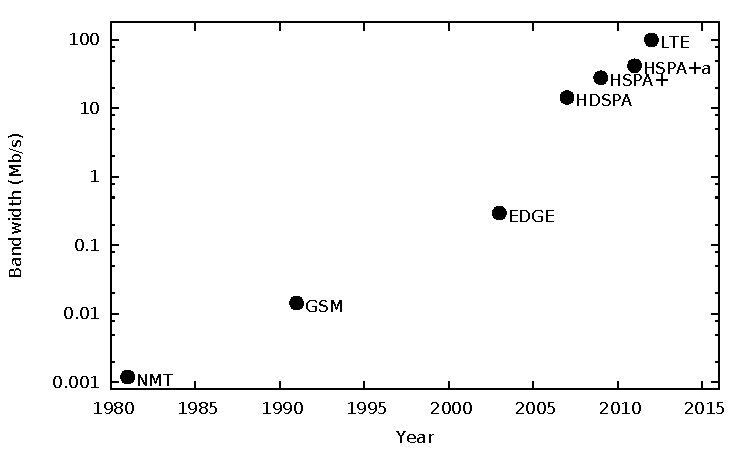
\includegraphics[width=0.99\textwidth]{img/charts/mobile-data-performance}
	\caption{
		Maximum download bandwidth available for mobile devices with time.
		%
		Each point is labelled with the specific communication technology name.
		%
		For the most recent multiple-input-multiple-output (MIMO) technologies, such as LTE, a conservative single input channel was used.
	}
	\label{img:mobile-bandwidth}
\end{figure}

The possibility of accessing the Internet from everywhere is probably one of the key bricks that allowed for the huge success of smartphones in today's world.
%
As \Cref{img:mobile-bandwidth} shows, the bandwidth available grew exponentially with time, to the point that in some countries (e.g. in Italy, at the time of writing) the best available mobile connections offer a higher performance than the best available home connection
%
\footnote{At the time of writing, Telecom Italia Mobile offers mobile connections on LTE with a download bandwidth up to 225Mb/s.
%
Fastweb, the company offering the faster solutions for fiber-to-home connections, goes up to 100Mb/s.}.
%
Such performance unlock the possibility of fully exploiting the possibilities of the world wide web, including cloud services and fruition of multimedia content.

If bandwidth is not currently an issue for international mobile telecommunications, the situation is well different when it comes to device density.
%
Any of us probably experienced network availability issues when participating crowded events, such as concerts or sport events.
%
The current technology, in fact, makes all the network user share the same physical resources: when the device density is too high, there is simply not enough space in the frequency spectrum to grant a decent bandwidth to everyone.
%
Future networks (5G, and presumably those that will follow) are focussing toward this issue among others \cite{5g}.
%
In particular, a so-called ``spectrum crunch'' is expected due to the expected traffic increase (thousand fold over this decade and still growing into the next), that could not be faced simply with the foreseen steady increase of the spectrum allocated for mobile communication, and will require technological advances \cite{spectrum-crunch}.

\subsection{WiFi}

WiFi technology is the most diffused technology for wireless local networking.
%
It is widely diffused, integrated in all smartphones and tablets and also in other devices, such as printers, gaming consoles and TVs.
%
WiFi devices communicate on a distance that ranges from 20 to 100 meters, depending on the condition of the wireless medium and on the power of the communication devices.
%
The communication speed between two linked devices ranges from 56Mb/s to 300Mb/s.

WiFi was designed to provide wireless access to a local area network.
%
In the most classic ``infrastructure mode'', wireless devices get connected to a so called access point, which is responsible to route packets among wireless devices and bridge the wireless local area network to the wired backbone.
%
Multiple access point that share the network name (SSID) may be connected using wired network technologies, and they will appear as a single, bigger access point.
%
It is also possible to drop the wired backbone, but specific access points are required.

Also, some WiFi devices provided ``ad-hoc mode'', allowing multiple devices to directly communicate without an intermediate access point.
%
This working mode was problematic, mainly due to the fact a standard communication protocol for peer-to-peer WiFi communication was missing.
%
This lack was filled with WiFi Direct, which provides a protocol by which one of the devices that want to communicate directly becomes the access point, allowing for direct communication.
%
The most common usage of such a feature are direct file sharing between devices and connection to peripheral devices such as printers or scanners.

\subsection{Bluetooth and Bluetooth LE}

Bluetooth is a technology designed for building energy efficient personal area networks (PANs).
%
Bluetooth devices are assigned a class which identifies the maximum permitted power and, consequently, the maximum operating range.
%
For the most powerful (and power hungry) devices the communication range can go up to 100m.
%
The communication speed ranges from 1Mb/s of the earliest 1.0 version to the 24 Mb/s of version 3.0 and later.

The most interesting features of Bluetooth are not the bandwidth nor the range (WiFi performs better on both), but rather the simple association process and the low power consumption.
%
Thanks to those features Bluetooth found widespread diffusion as a mean to connect low consumption peripherals, such as headsets.
%
Also, it is diffused in cars, and allows user to use the car's audio system as a speakerphone for making calls or listen to music.

\begin{figure}
	\centering
	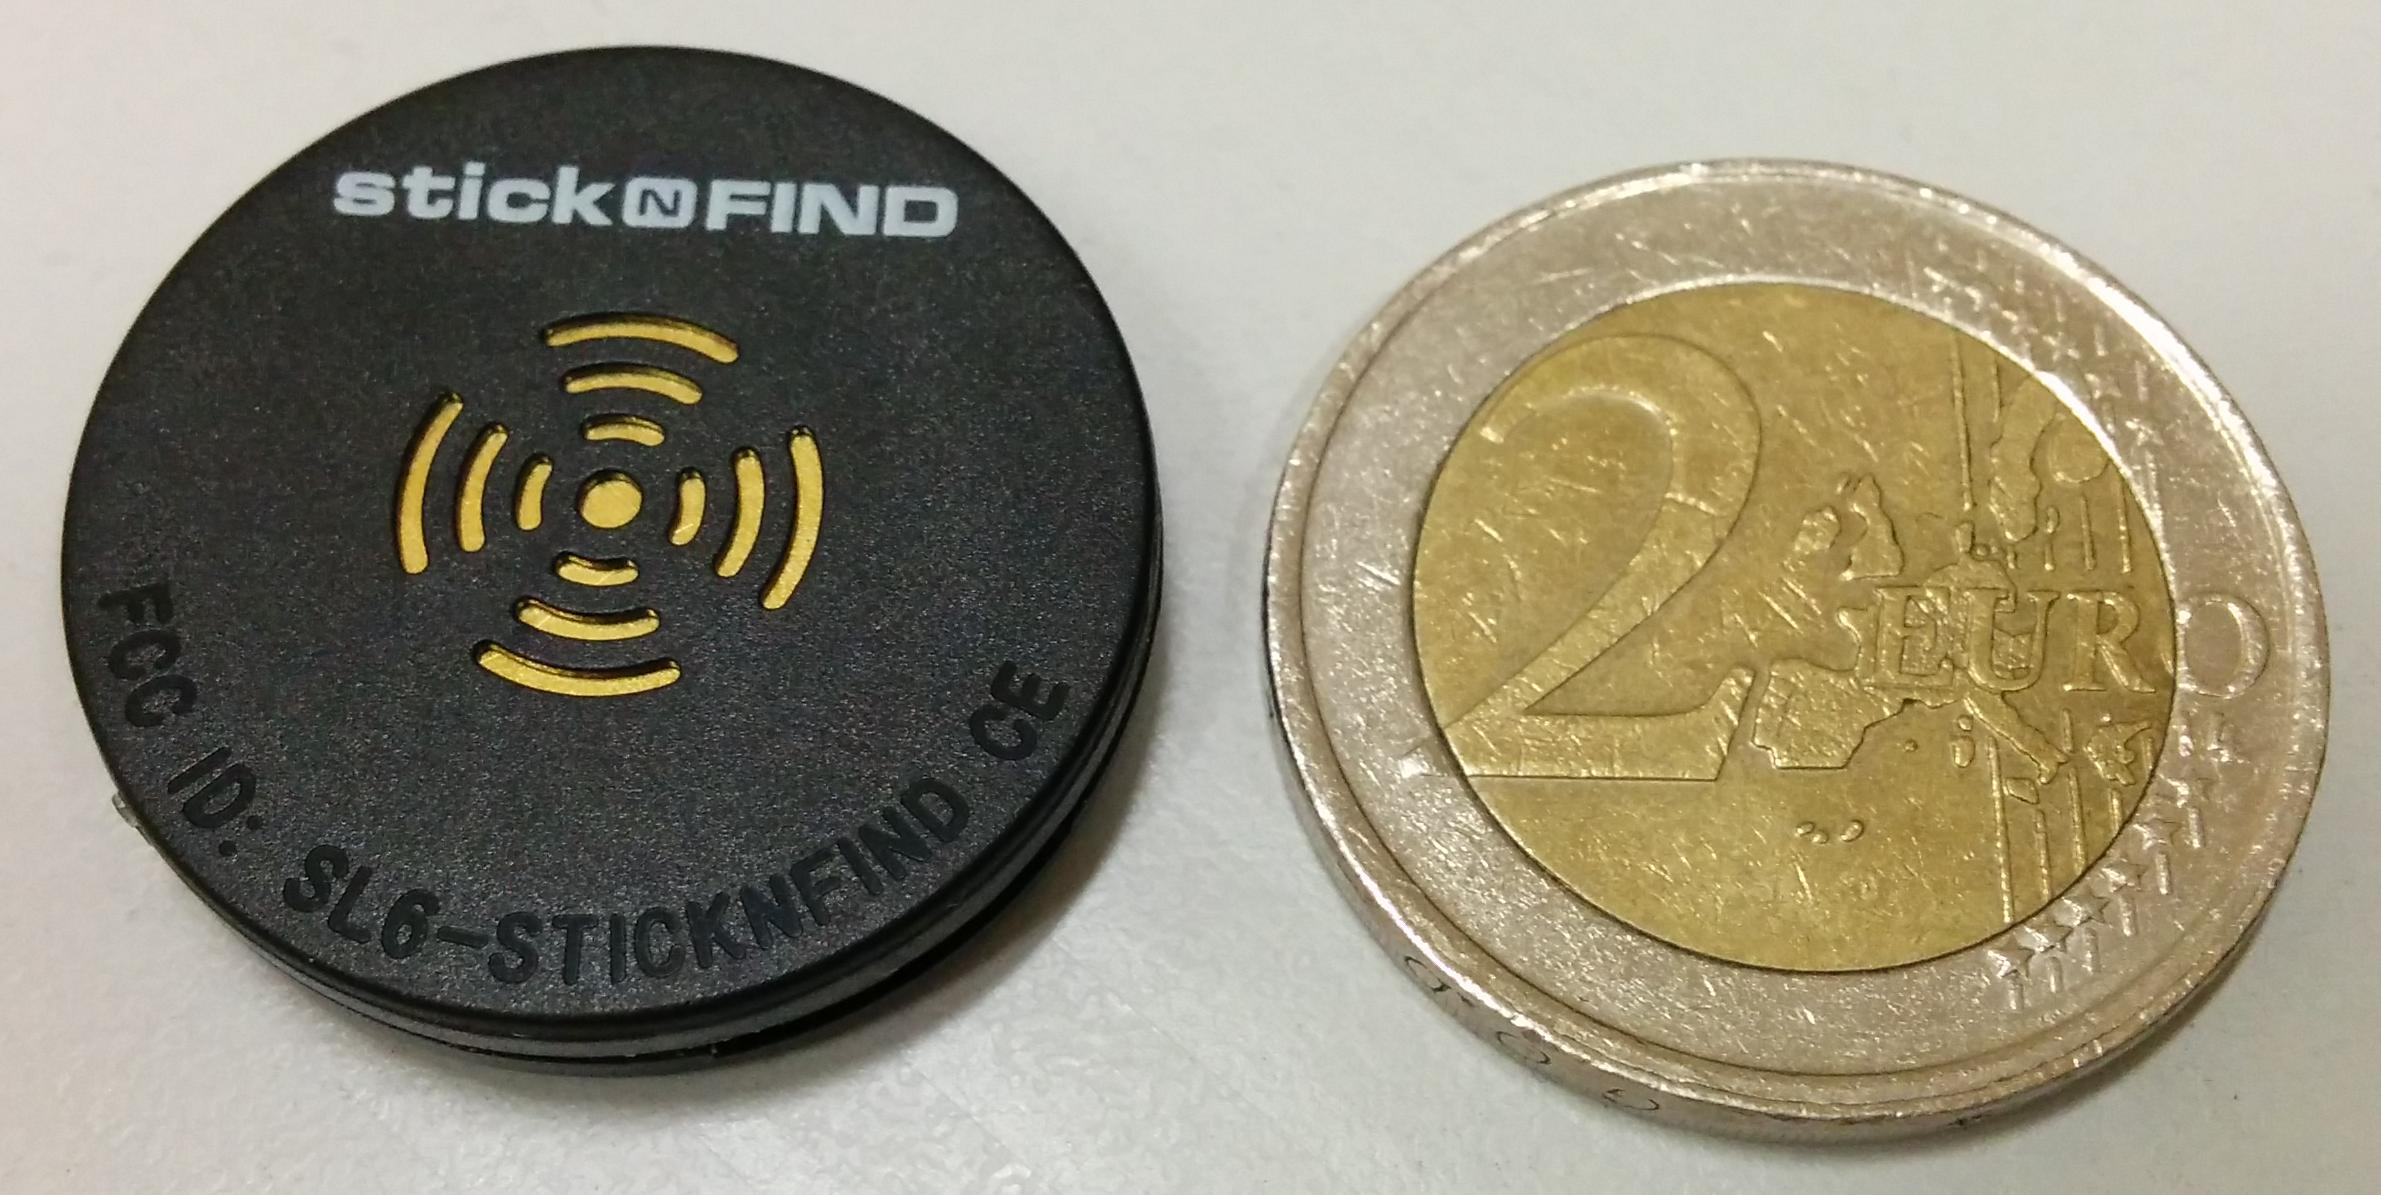
\includegraphics[width=0.99\textwidth]{img/ibeacon}
	\caption{
		A iBeacon, compared to a \EUR{2} coin.
	}
	\label{img:ibeacon}
\end{figure}

A technology which is often associated with Bluetooth but that is actually a separated and not compatible protocol is Bluetooth LE.
%
The reason why such technologies get associated is that, since the radio frequency used is the same (2.4GHz), dual mode devices can share a single radio antenna.
%
LE stands for Low Energy, and it is the main difference between the two protocols: at the expense of some bandwidth, Bluetooth LE consistently reduce the amount of energy required.
%
Bluetooth LE applications are particularly interesting, and range from health care to fitness to alerts to proximity sensing.

Proximity can be estimated using the received signal strength indicator (RSSI), and the very low power consumption of Bluetooth LE allowed for the realisation of electronic leashing systems, namely systems where an electronic device is paired to an object and can be used in order to compute the relative position.
%
The applications are, for instance, finding of misplaced, out-of-sight devices (when the electronic device is paired with a movable object) and indoor localisation (if the electronic device is located on a still standing object).
%
Relying on this technology, Apple created iBeacon, namely very small (coin sized, see \Cref{img:ibeacon}) electronic devices consisting basically of a battery and a Bluetooth LE device.
%
iBeacons can be attached to objects, and they send a universally unique identifier (UUID) to enabled smartphones in range.
%
If the smartphone can associate the UUID with a position, it can deduce its location relative to the iBeacon.
%
The low energy feature plays a fundamental role in this kind of applications: beacons whose battery would last few hours would be of little practical use.
%
With current technologies, a beacon device can be powered by a standard, rather cheap battery for several months, up to a couple of years.
%
This technology is probably the prelude to precise indoor localisation. 

\subsection{NFC}

\begin{figure}
	\centering
	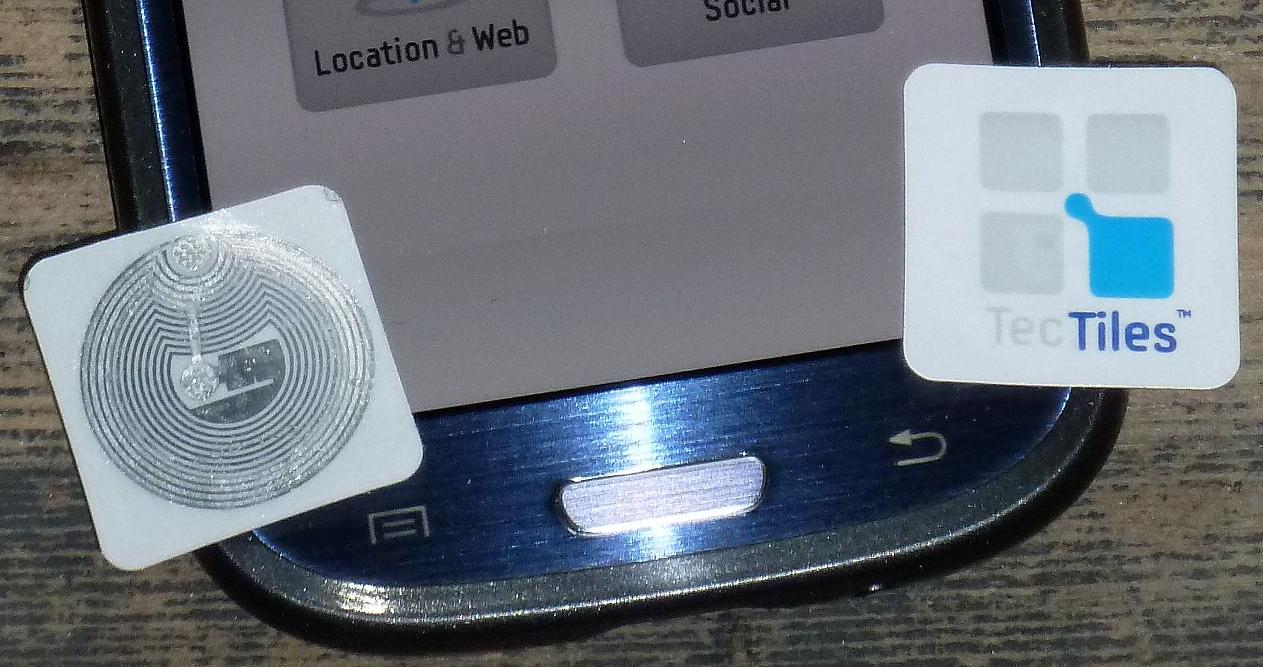
\includegraphics[width=0.99\textwidth]{img/nfc-tag}
	\caption{
		Two NFC tags, mounted on stickers.
		%
		In order to understand the size, they are placed above a Samsung Galaxy S3, a 4-inches smartphone.
		%
		Moreover, smaller versions of such tags exists, the models pictured here are very common-sized.
	}
	\label{img:nfc-tag}
\end{figure}

Near Field Communication, or NFC, is a technology designed for low energy communication between two devices in proximity (typically few centimetres).
%
It is designed for low energy consumption rather than high bandwidth: its speed (depending on the specification) ranges from 126kb/s to 242kb/s.

One of the most interesting features of NFC is that one of the two devices (the so-called ``tag'') can be completely passive, and still carry a small amount of information within (currently between 96 and 4096 bytes).
%
No battery or energy source is required, the information included can be read by active NFC devices in proximity.
%
Having no need of battery at all, NFC tags can really be tiny, even smaller than iBeacons.
%
\Cref{img:nfc-tag} shows two NFC tags: compared with iBeacons, they can be much lighter and thinner.
%
Brought to the world of humans, it is something like creating a sticker with very small sized text: those who have a powerful enough magnifying glass and are close enough to use it properly can read what it says.

The range of applications of such technology is rather broad.
%
The one which was probably most sponsored is contact-less payment, namely the ability to pay just tapping the phone close to the check-out counter.
%
This is a very interesting possibility, and indeed in 2007 there were enthusiastic forecasts \cite{nfc2007} about its quick diffusion, that did not happen as quick as expected.
%
A number of studies tried to understand the reasons behind this slow adoption, and it appears that reasons are more correlated to marketing and management rather than technological maturity \cite{nfc-diffusion-reasons, nfc-diffusion-europe, nfc-diffusion-asia}.
%
Similarly, if the phone stores identity or access tokens, NFC is a very suitable technology for effectively using such tokens: in this case, its very low range is a nice feature.
%
NFC can also be used as a technology enabler, namely as a mean to securely bootstrap another connection, or join a local network of devices.
%
An example of such use is the Android Beam technology, that relies on NFC in order to establish a Bluetooth connection between two Android devices, transfer a file, then close the Bluetooth connection.
%
Technically, NFC could be used to directly transfer files, but both WiFi and Bluetooth offer much wider bandwidths and range, and as a consequence are preferred for such task.
%
Another interesting application field is mobile device automation: it is achieved by attaching
%
Generally speaking, NFC comes in handy when there is need of a communication mean whose range should be very limited.


\section{Towards a P2P world?}

We are living exciting times.
%
In about five years from the introduction of the technology on the market, almost everybody got a personal smart device always with her.
%
Miniaturisation and power efficiency is constantly growing at a stunning rate, allowing data, communication systems and computation to be spread around in our physical world.

In few decades, we will probably witness the diffusion on computation on everyday object.
%
In such a scenario, the device density will be much higher if compared to the current.
%
One of the possible strategies is to connect every single device to the Internet, aggregate its information in a remote server, do the necessary computation, then send back eventual results where they are needed.
%
This is the strategy behind cloud computing, which is achieving great success.
%
In particular, I argue, this strategy is interesting when the information could or should be aggregated with information from other, distant sources, or conserved for historical purposes.
%
This path, however, gets harder and harder to follow when device density increase: besides the obvious increasing on the total information produced, and consequently of the information to transmit and process, there are two other problems: the saturation of the wireless medium, and the locality of information.

Who tried to use its own smartphone in a very crowded environment has probably experienced connection or network issues.
%
The problem, as discussed in \Cref{International Mobile Telecommunications}, is that current technology must share a common medium among all the devices in the same area.
%
Increasing the maximum number of devices per area is one of the goals of the next generation of international mobile telecommunication technologies.
%
One of the proposed approaches is to switch to a very dense array of very small cells by deploying multiple antennas at a very short distance one another, e.g. inside the public illumination poles.
%
Devices nearby the local antenna would connect to it, and the antenna would then connect them to the rest of the network transparently, in a way somehow similar to the current WiFi ``infrastructure mode''.
%
Clearly, diffusing such antennas can possibly represent a major infrastructural upgrade, and, potentially, cost.

Another observation is that not every device needs direct access to the Internet to be able to accomplish its task, and this is increasingly true with increased density.
%
Thinking about today's devices, let's consider the current smartwatches and fitbands: the former relies on a smartphone or tablet in order to provide Internet-based services, and the latter uses no Internet connection at all, but just sends data to the smartphone to be processed.
%
Along the line of favouring locality, there is a second advantage which relates to privacy issues: there is no reason to send personal information away, if the system does not need data from distant points nor requires more computational power of the amount available locally.
%
Privacy issues gain great attention recently, especially after the leaks of classified information started in 2010 on Wikileaks and continued with the more recent leaks by Edward Snowden.
%
The content of such documents raised greater attention to privacy issues from general public.

A possible path which would help in both those directions (reduce wireless medium usage and keep data as local as possible) is the usage of local, possibly peer-to-peer interactions.
%
This way of organising communication is already exploited by existing applications.

One notable example is Firechat \footnote{\url{https://opengarden.com/firechat}}, which got particularly spotlighted during the ``Umbrella revolution'', namely the sequence of protests that took place in Hong Kong in 2014.
%
Similarly to what was done during Arab springs in 2011 \cite{arab-spring}, protesters relied on Internet services to organise and coordinate themselves.
%
The Chinese government policy on internet is not exactly a bright example of openness and neutrality \cite{china-censorship}, and services such as Facebook adn Twitter, widely exploited during Arab springs, were already effectively blocked in the land.
%
In short time, other social network were closed (such as Instagram), in order to cut protesters' communication means.
%
At that point, protesters had to find a communication system free of centralisation in order to prevent targeted Internet filters, and Firechat was the answer.
%
Firechat is a messaging application for mobile phones that, when the smartphone has access to the remote Firechat cloud, works as other more famous alternatives, such as WhatsApp\footnote{\url{http://www.whatsapp.com/}} and Telegram\footnote{\url{https://telegram.org/}} do.
%
When no access to Firechat servers is available, then the software tries to reach the destination by spreading the message hop-by-hop, building a de-facto mesh network.

Another interesting experiment is Serval Mesh \cite{serval-mesh}.
%
Serval Mesh accomplishes similar tasks, but it also supports calls and file transfers besides messaging.
%
Its main goal is to provide a networking among users who are in an area where there is no Internet access at all, for instance because of a disaster event.
%
It relies on WiFi to create a ad-hoc peer-to-peer network among devices.
%
Due to this lower level aspect, Serval Mesh requires privileged access to the hardware and some higher skill than Firechat, which is easier to setup but requires the availability of a Internet connection.
%
In \cite{mesh-network-telephony}, Serval Mesh is used to build an alternative, purely peer-to-peer telephony network.

Despite the existence of such mesh-oriented applications, however, a general approach for easily design and program such systems is still missing.
%
A consistent part of this work is devoted towards the research of general, well engineered approaches to build such systems.

\chapter{Coordination infrastructures}

In \Cref{pervasive-devices} we took a look to the world of pervasive devices, also describing their communication means and hypothesising the near future development.
%
In this chapter, we focus on the software, and in particular on the challenges of engineering the development of software that will run on 

\label{coordination-infrastructures}
\section{The issue of coordination}
why do we want a middleware
\section{Nature inspiration}
see what exists, mimic
\section{Coordination platforms and languages}
what is there already
\subsection{Linda}
and swarmlinda
\subsection{TOTA}
\subsection{TuCSoN}
and the semantic extension
\subsection{Biochemical tuple spaces}
and MoK?
\subsection{SAPERE}
general idea of sapere, grounds on previous works.
\subsection{Proto and Field Calculus}
\subsubsection{Alignment}
\section{Spatial patterns}
what is a pattern
patterns before sapere (gossip, gradient)
problems with gradient
\section{Engineering and tools}
methodological issues, deployment and testing issues, need of simulation
\subsection{General purpose frameworks}
Repast, netlogo
\subsection{Specific simulators}
network simulators (the one, ns2)
biological simulators (ask Sara)

Specific per-use simulators, gener

% \part{Motivation}
\chapter{Shortcomings of coordination infrastructures}
\section{Engineering emergence}
\section{Local to global}
\chapter{Shortcomings of existing tools}
\section{Specific tools: expressiveness}
\section{General purpose tools: performance}

\part{Contribution}
\label{contribution}
\chapter{Integrated tools for designing pervasive ecosystems}
\section{Chemical inspired MABS}
\section{Meta-meta model}
\section{Chemical meta-model}
\subsection{Simulation of a morphogenesis model}
\section{SAPERE meta-model}
\section{Advanced features}
\subsection{Distributed statistical analysis}
\subsection{Real world maps}

\chapter{Self-organisation patterns}
SAPERE
\section{Crowd evacuation}
\section{Self composition}
\section{Semantic resource discovery}
\section{Anticipative adaptation}
\section{Crowd disasters prediction}
\section{HPC at the urban scale}

\chapter{Aggregate programming languages}
Protelis
\section{Higher order functions in field calculus}
\subsection{Impact on alignment}
\section{Java integration}
\section{Alchemist as a simulation platform}
\section{Alchemist as a core engine for real devices}

\part{Conclusion}
\chapter{Results achieved}

\chapter{Future and ongoing work}
\section{Biochemical meta model for Alchemist}
ciao

%\appendix
%\input{appendix-a.tex}
%\input{appendix-b.tex}
%\input{appendix-c.tex}

%\input{publication.tex}

\part{Bibliography}

%===============================================================================
\small\protect\newpage\addcontentsline{toc}{chapter}{Bibliography}
\bibliography{thesis}
\bibliographystyle{alpha}
%===============================================================================

%\listoffigures
%\listoftables

\end{document}
